\documentclass{article}

% if you need to pass options to natbib, use, e.g.:
\PassOptionsToPackage{numbers, compress}{natbib}
% before loading neurips_2019

% ready for submission
% \usepackage{neurips_2019}

% to compile a preprint version, e.g., for submission to arXiv, add add the
% [preprint] option:
%     \usepackage[preprint]{neurips_2019}

% to compile a camera-ready version, add the [final] option, e.g.:
     \usepackage[final]{neurips_2019}

% to avoid loading the natbib package, add option nonatbib:
%\usepackage[nonatbib]{neurips_2019}
\usepackage{subfigure}

\usepackage{graphicx}
\usepackage{hyperref}
\usepackage{float,flafter}
\usepackage[utf8]{inputenc} % allow utf-8 input
\usepackage[T1]{fontenc}    % use 8-bit T1 fonts
\usepackage{hyperref}       % hyperlinks
\usepackage{url}            % simple URL typesetting
\usepackage{booktabs}       % professional-quality tables
\usepackage{amsfonts}       % blackboard math symbols
\usepackage{nicefrac}       % compact symbols for 1/2, etc.
\usepackage{microtype}      % microtypography

\title{Detecting face mask by using machine learning}

% The \author macro works with any number of authors. There are two commands
% used to separate the names and addresses of multiple authors: \And and \AND.
%
% Using \And between authors leaves it to LaTeX to determine where to break the
% lines. Using \AND forces a line break at that point. So, if LaTeX puts 3 of 4
% authors names on the first line, and the last on the second line, try using
% \AND instead of \And before the third author name.

\author{%
  Yong Yu\\
  University of Victoria\\
  \texttt{yongyu1@uvic.ca} 
}

\begin{document}

\maketitle

\begin{abstract}
  The face mask has become a daily essential for us since pandemic, we are required to wear them in any public area, but more importantly, we want to make sure other people are doing it. We want to make sure they have their mask on as well.
In this paper, we addressed three different machine learning models to solve this problem, where we can detect if a person is wearing a mask or not by our models through the camera.


\end{abstract}

\section{Introduction}

As we addressed the problem shown in the abstract section. We will first talk about the problem and our motivation. Then, we will talk about the dataset used to train and test our models. For the dataset, we will have some preprocessing steps we need to take before we can use them in training. \\
We will give some introduction about the convolutional neural network and residual network. We will use both of them in the project. Then we will introduce the transfer learning technique, which allows us to adapt knowledge from the existing models.\\
We will describe the models we built in detail, including training time, train accuracy, test accuracy, and the models’ architectures.\\
Finally, we will discuss the result, show the confusion matrix, and reported the best model base on the test accuracy.




\section{Problems}
\label{gen_inst}
The problem is trying to detect if a person is wearing a mask or not. In terms of machine learning, this is a binary classification problem, where the output for our model will be 0 or 1, in this project, 1 as if the person is wearing a mask, 0 otherwise. \\
We want to take advantage of machine learning to accomplish this problem. We will be building machine learning models and training them with our dataset. 
\subsection{Motivation}
We want to do this project because of a few reasons. First, we will build the models that were not covered in class. We will describe them in the background section. The second reason is we want to gain more experience with computer vision problems, primarily if we can interact with, such as this project, it this project. What we need are a webcam and a face mask. The third reason will be this is such a trending topic, maybe not in a good way. This model has many real-world usages. For example, put it on the front door of the house. 

\subsection{DataSet}
In this project, we are using the dataset provided in the following URL:
\begin{center}
\url{https://data-flair.training/blogs/download-face-mask-data/}
\end{center}
This dataset contains 1376 images in total, with 690 images containing images of people wearing masks and 686 images with people without masks. After we obtain the dataset, we will have to preprocess the dataset before we use them directly in training. We have to do some preprocess steps.\\
\begin{itemize}
\item \textbf{Grayscale images: }We will load the dataset images as gray scale images, the color doesn't provide any helpful information when detecting face masks in the pictures. Colored are more complex for computers.
\item \textbf{Resize the images: }By making sure our model is consistent, we make sure, all the data has the same shape. We will shape our data as (224, 224, 3). We will discuss why we resize them to this size next section when we talk about the pre-trained models we will use in this project.
\item \textbf{Data augmentation: }We increase the size of the dataset by rotating them by [90, 270] degrees, we will end up with a dataset tripped the size of the original dataset. Our dataset now contains 4128 samples.
\item \textbf{Labeling: }The original dataset provided all the images. However, when we doing supervised learning, we need to label the data ourselves, we will label the images with the facemask with 1 and images without face mask with 0.
\item\textbf{CSV: }In order to access the images and the transformation from the code, we need to be able to store the data in some manner. We choose to store the data in a CSV file containing the following information:
	\begin{enumerate}
	\item The path to the image.
	\item The label of the image.
	\end{enumerate}
\end{itemize}
Now we have the dataset that can be easily access with codes. We choose some sample images shown in Figure 1.
\begin{figure}[H]
 \centering
    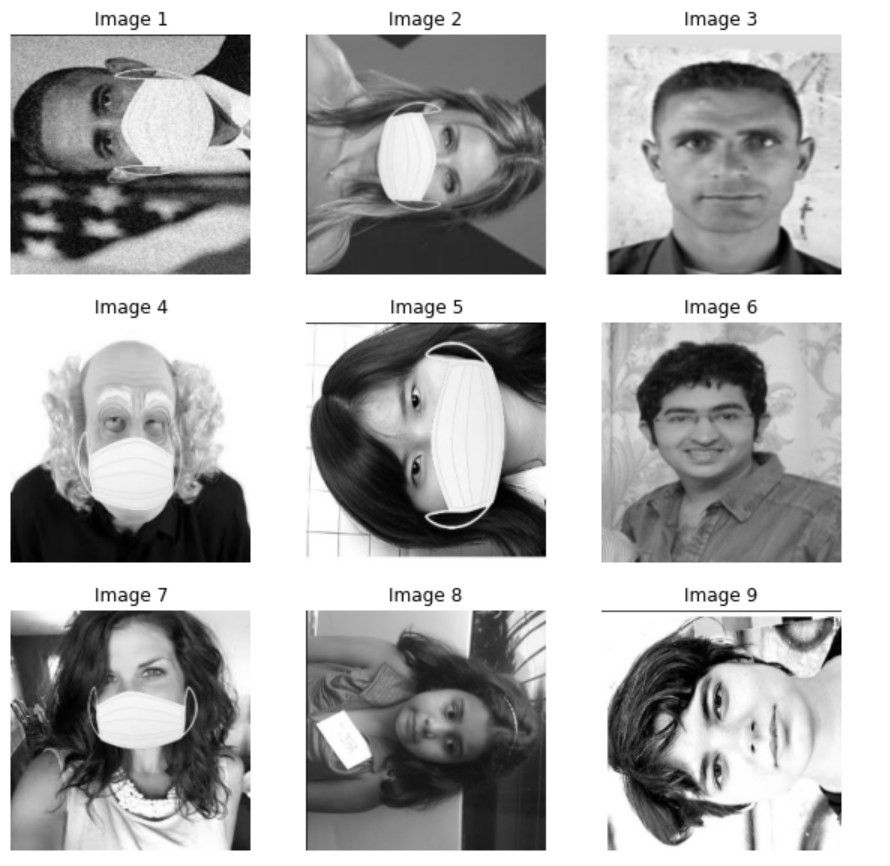
\includegraphics[width=3.0in]{figs/samples}
    \caption{Samples}
    \label{Samples}
\end{figure}


\section{Background}
\label{headings}

 To better understand the project, the model, and the concept we used. This chapter provided a background introduction to two different neural networks which are convolutional neural networks and residual neural networks. We will explain the concept of transfer learning, which allows us to adapt the knowledge from an existing model so we will need much less data to get a good result.
\subsection{Convolutional neural networks(CNN)}
  A convolutional neural network(CNN)\cite{albawi2017understanding} is known to be good when dealing with image tasks. A basic convolutional neural network includes four different types of layers. They are convolutional layers, pooling layers, fully connected layers, and output layers. We show the architecture of a convolutional in Figure 2.

\begin{figure}[H]
 \centering
    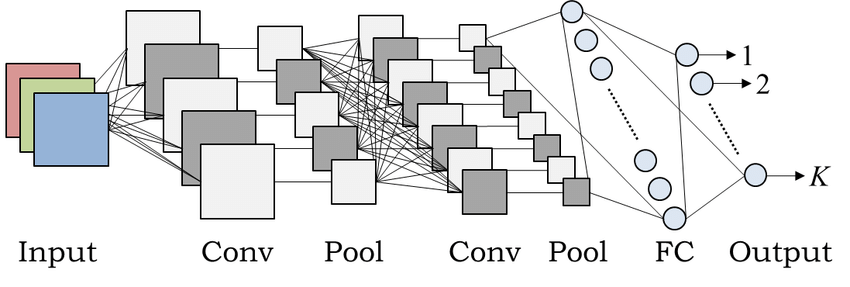
\includegraphics[width=3.0in]{figs/cnnArch}
    \caption{CNN architecture}
\end{figure}.

We will give a brief introduction of each layer about what they do.\\
\textbf{Convolutional layer: }The convolutional layer applies different filters to the input. The earlier convolutional layers identify the simple features such as horizontal/vertical lines, corners dot... later convolutional layers identity more complex features. There are two different parameters we can set in this layer, padding, and strides. We can choose using ‘same’ padding or ‘valid’ padding. One of them shrinks the size of the input image after the filter, one of them not. The stride is an integer that tells how many pixels the filter will move each time. \\
\textbf{Pooling layer: }In general, the pooling layer will shrink the input size but try to keep its features, we can choose to do max-pooling or average-pooling. For each region represented by the filter, we take the max/average of that region and create a new, output matrix where each element is the max/average of a region in the original input. That is the different between max/average pooling.\\
\textbf{Fully connected layer: }The fully connected layer is like a layer we will see in a typical neural network. It is the output from the final pooling or convolutional layer. \\
\textbf{Output layer: }We will output the result in this layer.

\subsection{Residual neural networks}
The original paper of residual network came out at 2016\cite{he2016deep}. When people are still training 20~30 layers models, the authors of this paper\cite{he2016deep} came out with the architecture of the residual neural networks around about 50 layers and still holds good accuracy impressive. \\
The residual neural network is often much deeper than a convolutional neural network, but that doesn’t mean we need to train as many parameters. The residual neural network introduces the architecture call residual blocks shown in Figure 3.
\begin{figure}[H]
 \centering
    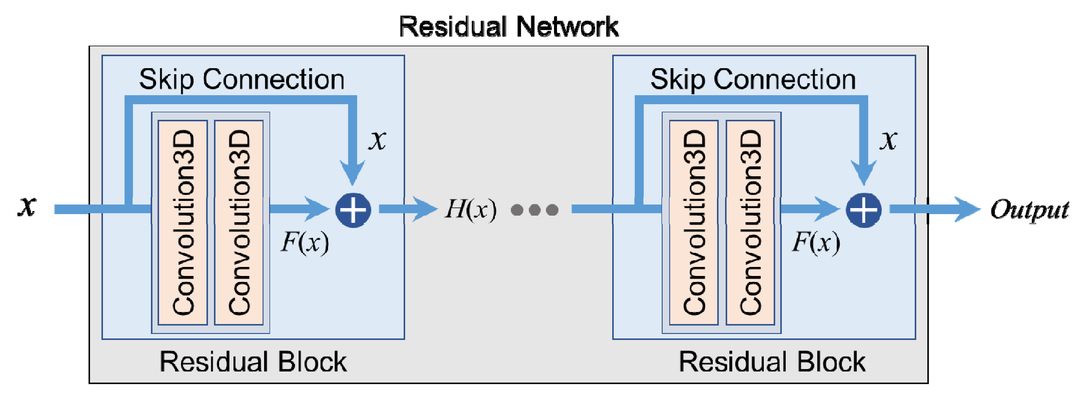
\includegraphics[width=3.0in]{figs/resblock}
    \caption{Residual block architecture}
\end{figure}
Unlike a traditional neural network where we pass the input layer by layer, the residual network has some skip connections.

\subsection{Transfer learning}
Transfer learning\cite{pan2009survey} can be very helpful with certain machine learning or data mining model. Transfer learning allows us to use the knowledge within a neural network that has already been trained and apply it to help solve a new task. That means we can find a neural network that is has been trained to do some task. We strip off the last few layers in the pre-trained neural network and add our own customized layers after that so that when we train the neural network, we only need to train the new layers that we added while retaining the knowledge of the other layers.\\
The problem of building and training a model from scratch is that sometimes it is too hard or is impossible to collect enough data for the model, or it takes too much resources to train and build the model from scratch. By using transfer learning, we may avoid these expenses. Transfer learning can be applied to different machine learning problems.\\
In transfer learning, we find a pre-trained machine learning model and we only keep the
part that we need to keep in the model, and we add some new layers after. We only
need to train the layers that come after the original model, which can save data and
time. Figure 4 shows briefly how transfer learning works.
\begin{figure}[H]
 \centering
    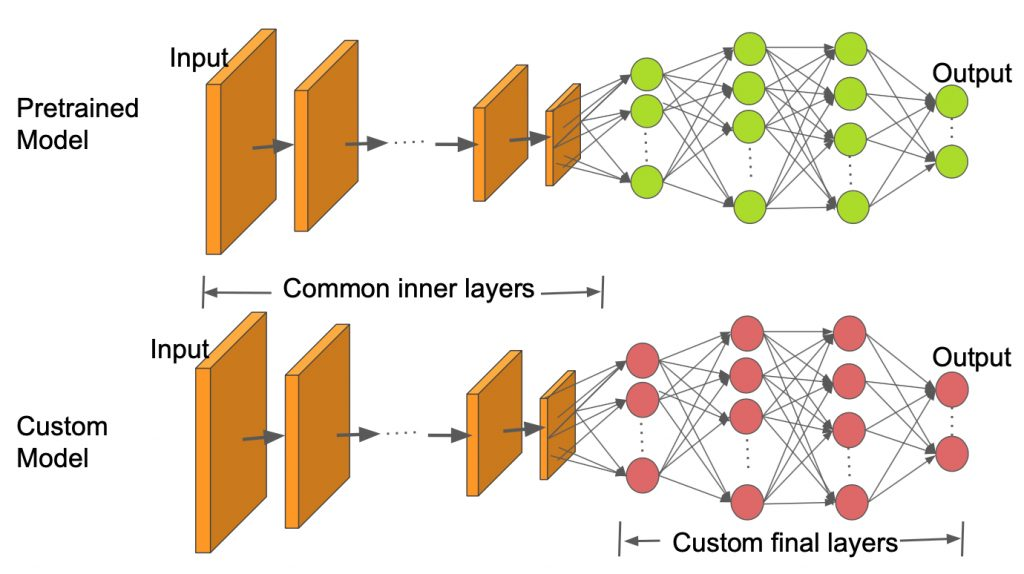
\includegraphics[width=3.0in]{figs/transfer}
    \caption{Transfer learning}
\end{figure}
In this project, we will build two models that take advantage of transfer learning. One of them uses a pre-trained CNN, and another one uses a pre-trained ResNet(residual network). We will introduce them in the next section.

\section{The models}
\label{others}
This section will give a more detailed description of our models. There are three models we will be built. Two of them take advantage of transfer learning. We have found two pre-trained models that we will use, called VGG16\cite{simonyan2014very} and ResNet50\citep{he2016deep}.We showed the architecture of the models in Figure 5.\\
The VGG-16\cite{simonyan2014very} is a 16 layers pre-trained convolutional neural network trained with over 40 million images. It takes the input image size of (224 x 224). \\
The ResNet50\citep{he2016deep} is a pre-trained residual neuron network that has total of 50 layers trained over million of images. It also takes the input image size of (224 x 224).

\begin{figure}[H]
    \centering
    \subfigure[]{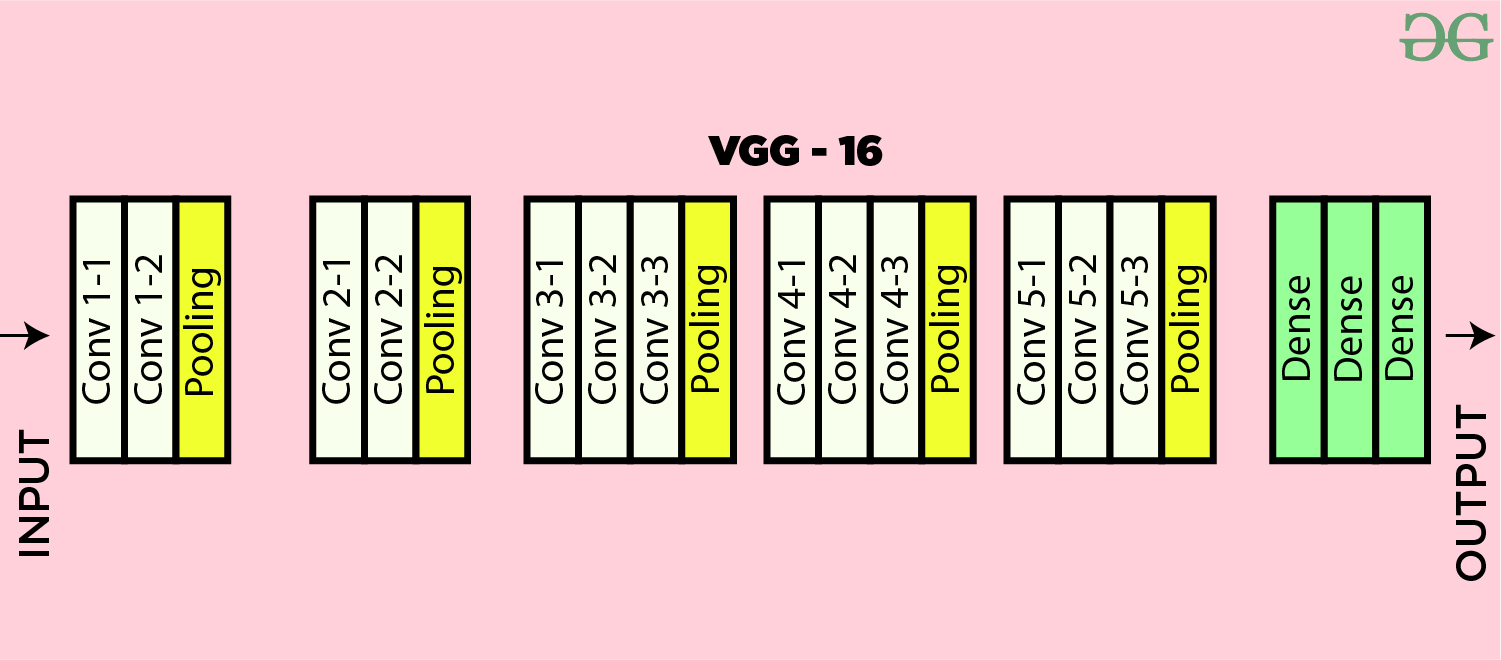
\includegraphics[width=3.0in]{figs/vgg16}} 
    \subfigure[]{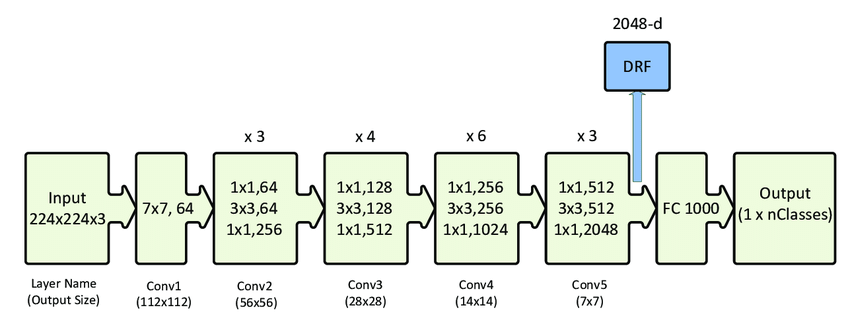
\includegraphics[width=3.0in]{figs/resnet50}} 

    \caption{(a)VGG16 architecture (b)ResNet50 architecture}
    \label{fig:foobar}
\end{figure}
\subsection{Base model}
The first model is a plan convolutional neural network. It has two convolutional layers with two max-pooling layers, followed by the fully connected layer, one dense layer, and the output layer. The architecture of the model is shown in Figure 6. It has a total of 24,190,209 parameters to train.
\begin{figure}[H]
 \centering
    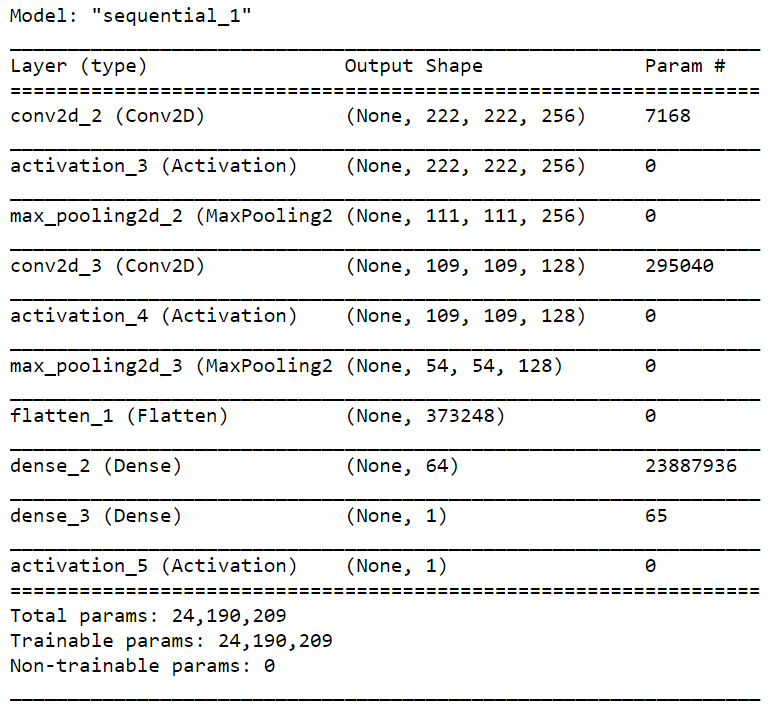
\includegraphics[width=3.0in]{figs/Model}
    \caption{Base model}
\end{figure} 

\subsection{VGG16 base model}
We build a model using transfer learning and uses the VGG16\cite{simonyan2014very} as a pre-trained model. We will freeze the weight of this model. We will not include the layers after the last layer of the convolution/pooling layer in the model. We added 2 dense on top of the pre-trained model and shown the architecture of this model in Figure 7. This model has 3,211,521 parameters to trained.
\begin{figure}[H]
 \centering
    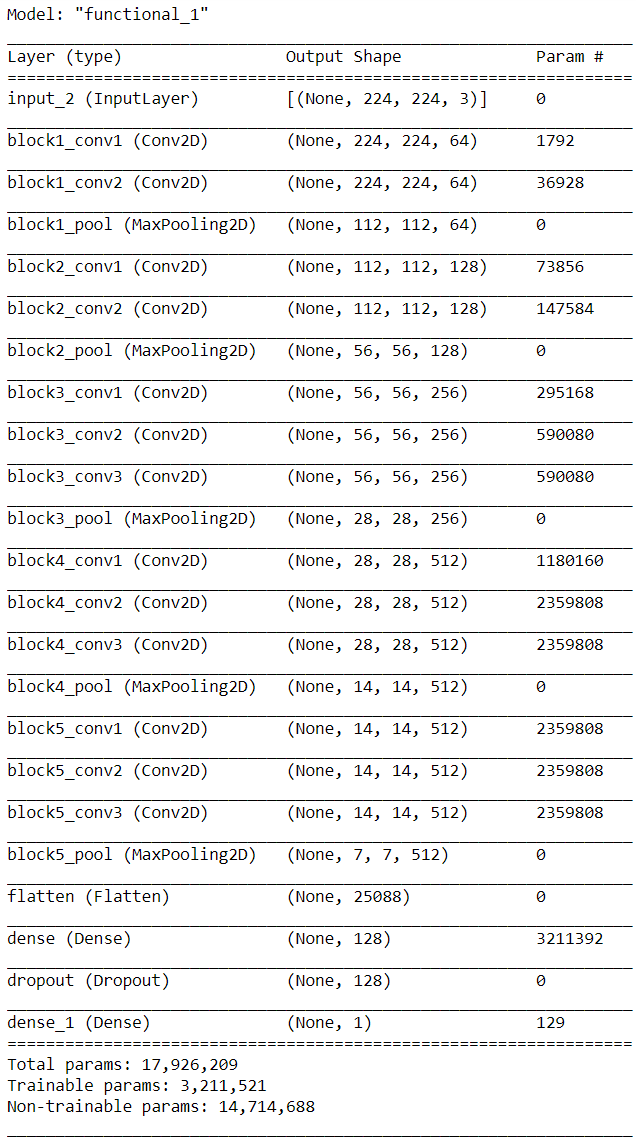
\includegraphics[width=3.0in]{figs/vggmodel}
    \caption{VGG16 model}
\end{figure} 

\subsection{ResNet50 base model}
Similar to the vgg16 model. This model uses ResNet50 as a pre-trained model, and it has 13,255,297 parameters shown in Figure 8.
\begin{figure}[H]
 \centering
    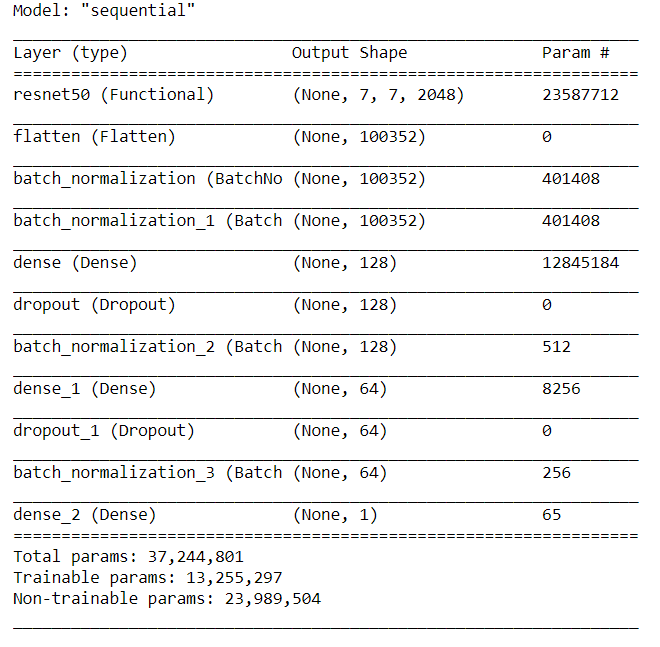
\includegraphics[width=3.0in]{figs/resnetmodel}
    \caption{ResNet50 model}
\end{figure} 

\section{Experiment and result}
This section describes how we set up this experiment and the experiment result.  
\subsection{Training}
After we preprocess our dataset. Our training dataset contains a total of 3939 samples. The test dataset sontains 579 samples. We will use 10\% of the data from training set as validation data. The new dataset size as describe as follow:
\begin{itemize}
\item \textbf{Train data: }3545 samples.
\item \textbf{Validation data: }394 samples.
\item \textbf{Test data: }579 samples.
\end{itemize}
Now we have the dataset, we will report the total training time that takes to train each model on an \textbf{i5 CPU}.
\begin{itemize}
\item \textbf{Base model: }3h 19min 14s.
\item \textbf{VGG16 base model: }2h 1min 10s.
\item \textbf{ResNet50 base model: }1h 42s.
\end{itemize}
\subsection{Result}
In this section, we will report the train and test accuracy for each model, and base on the accuracy, we pick the model with the best accuracy as the best model for our project.
\begin{itemize}
\item \textbf{Base model.}
	\begin{itemize}
	\item Train accuracy: \textbf{0.4996}
	\item Test accuracy:\textbf{0.4974}
	\end{itemize}
\item \textbf{VGG16 base model.}
	\begin{itemize}
	\item Train accuracy:\textbf{0.9939}
	\item Test accuracy:\textbf{0.9862}
	\end{itemize}
\item \textbf{ResNet50 base model.}
	\begin{itemize}
	\item Train accuracy:\textbf{0.8191}
	\item Test accuracy:\textbf{0.8497}
	\end{itemize}
\end{itemize}
Base on the train and test accuracy, the \textbf{VGG16 base model} has the highest accuracy for both train and test dataset. The \textbf{VGG16 base model} will be the best model to pick for this project.
\section{Conclusion}
We developed three different machine learning models to detect if a person is wearing a mask or not. We preprocessed the dataset for better training experiments.\\
We introduced two different neural network types, convolutional neural networks\cite{albawi2017understanding}
 and residual neural networks\cite{he2016deep}
. We also introduced the concept of transfer learning\cite{pan2009survey}
. Two of the models we built uses transfer learning. \\
We introduced two pre-trained models that we use during our implementation. VGG16\cite{simonyan2014very}
 and ResNet50\cite{he2016deep}.\\
We trained the models and picked the model for our problem, which comes out to be the VGG16 base model. We tested our model in real world and the result shown in Figure 9.
\begin{figure}[H]
    \centering
    \subfigure[]{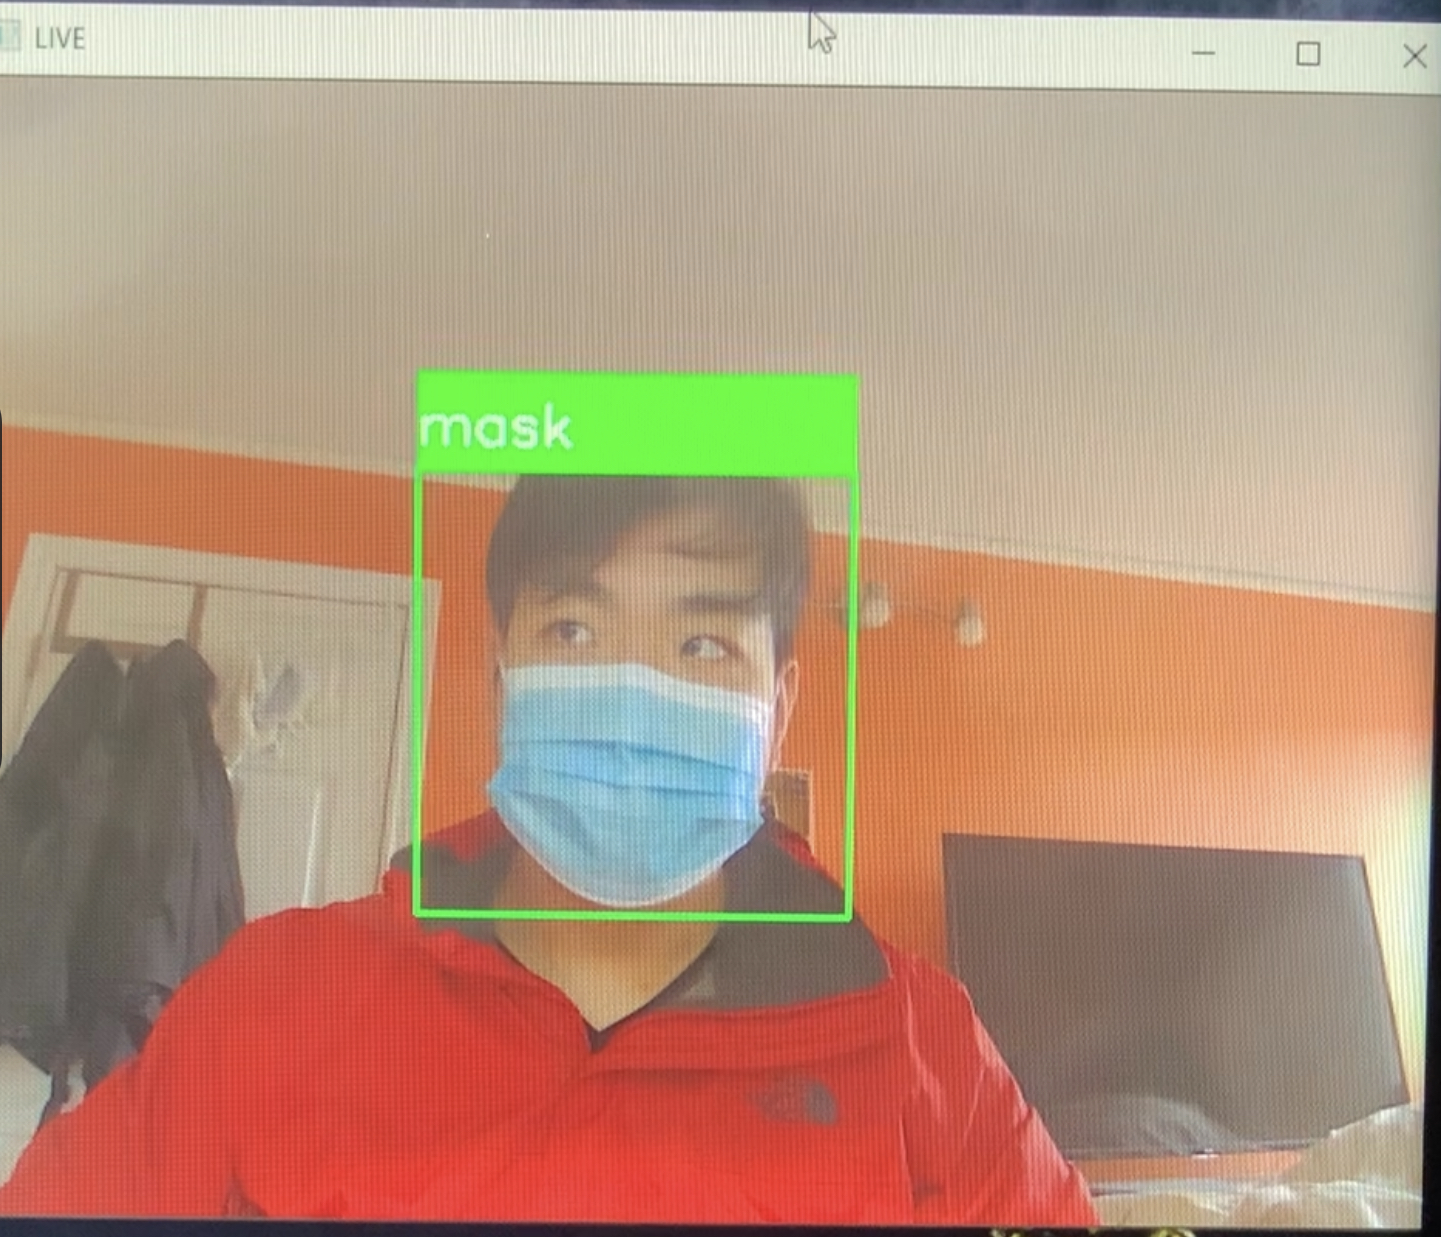
\includegraphics[width=3.0in]{figs/mask}} 
    \subfigure[]{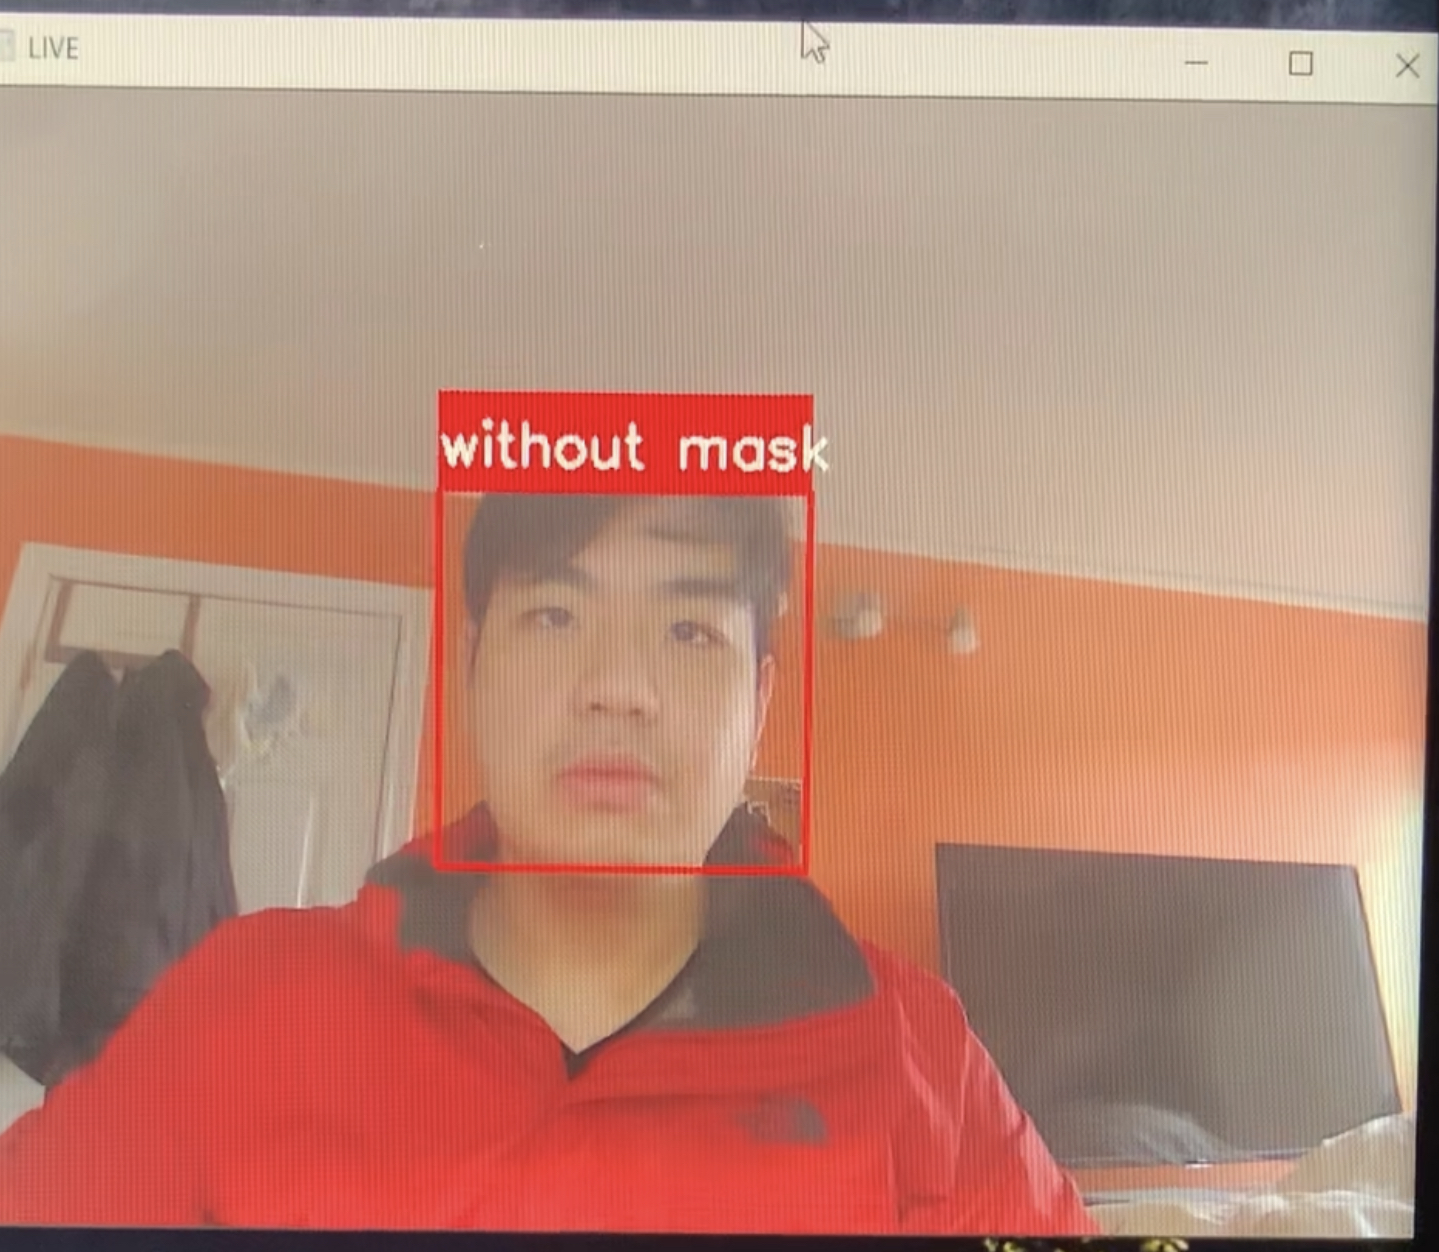
\includegraphics[width=3.0in]{figs/nomask}} 

    \caption{(a)With mask (b)Without mask}
\end{figure}
As we can see the model classify the images successfully. 
\subsection{Future work}
During the training time, I was using the cpu, so it takes a while to train, we can lower the training time by GPU or an online server such as AWS.\\
We can try to integrate the model into software as long we can access  with proper API.\\
The accuracy can be future improve by collecting more data or adding more layers to our models. We will need more resource to train them.

\bibliography{bibliography}
\bibliographystyle{acm}
\end{document}
